\documentclass[11pt,fleqn, a4paper]{exam}
\usepackage[utf8]{inputenc}

\usepackage[margin=1in]{geometry}
\usepackage{amsmath,amssymb}
\usepackage{gensymb}
\usepackage{multicol}
\usepackage{float}
\usepackage{graphicx}
\usepackage{units,icomma}
\usepackage{hyperref}
\usepackage{enumerate}
\usepackage{wasysym}
\usepackage{multirow}
\usepackage[usenames,dvipsnames]{xcolor}
\usepackage[margin=1.5cm]{caption}
%\everymath{\displaystyle}

\hyphenation{
  chro-no-ampe-ro-met-ric
  ber-dia-me-ter
  de-ngan
  me-nem-pati
  mic-ro-graphs}

\renewcommand{\figurename}{Gambar.}
\renewcommand{\labelitemi}{$-$}


\newcommand{\class}{OLIMPIADE ASTRONOMI}
\newcommand{\term}{Tingkat Provinsi - 2015}
\newcommand{\examnum}{OSP Astronomi 2015}
%\newcommand{\examdate}{11/02/2014}
%\newcommand{\timelimit}{120 Minutes}

\pagestyle{head}
\firstpageheader{}{}{}
\runningheader{\examnum}{}{Halaman \thepage\ dari \numpages}
\runningheadrule


\begin{document}

\noindent
\begin{tabular*}{\textwidth}{l @{\extracolsep{\fill}} r @{\extracolsep{6pt}} l}
\textbf{\class} \\% & \textbf{Name:} & \makebox[2in]{\hrulefill}\\
\textbf{\term}  %&&\\
%\textbf{\examnum} &&\\
%\textbf{\examdate} &&\\
%\textbf{Time Limit: \timelimit} & Teaching Assistant & \makebox[2in]{\hrulefill}
\end{tabular*}\\
\rule[2ex]{\textwidth}{2pt}

\noindent
\begin{tabular}{ll}
\textit{Copyright} (c) 2015 & Ridlo W. Wibowo (ridlo.w.wibowo@gmail.com)\\
                   & Sulistiyowati (sulis.astro08@gmail.com)
\end{tabular}

\vspace{0.3cm}
\noindent
Solusi ini dibuat tanpa jaminan kesesuaian dengan solusi resmi dari juri olimpiade sains bidang Astronomi. Pengguna boleh menyebarluaskan dan/atau memodifikasi solusi ini dengan mencantumkan sumber asli. Hak cipta soal ada pada Kemendiknas dan dilindungi undang-undang.

\vspace{0.4cm}
\noindent
\rule[2ex]{\textwidth}{1.5pt}

\textbf{Soal Pilihan Berganda}

\begin{questions}
\question Sistem bintang ganda Albireo terdiri atas dua buah bintang dengan magnitudo masing-masing komponen adalah 3,35 dan 5,9. Seorang pengamat mengamati sistem bintang ganda Albireo ini dengan mata telanjang. Terang sistem bintang yang terlihat adalah
\begin{choices}
\choice 2,55
\choice 3,25
\choice 4,63
\choice 5,90
\choice 9,25
\end{choices}

\textit{Jawaban: B}\\
$m_1=3,35$ dan $m_2=5,9$

\vspace{-0.75cm}
\begin{minipage}[t]{0.5\textwidth}
\begin{eqnarray*}
m_1-m_2&=&-2,5\log \frac{E_1}{E_2}\\
\frac{E_1}{E_2}&=&10^{\frac{m_2-m_1}{2,5}}\\
\frac{E_1}{E_2}&=&10,47
\end{eqnarray*}
\end{minipage}
\begin{minipage}[t]{0.5\textwidth}
\begin{eqnarray*}
m_{tot}-m_2&=&-2,5\log \frac{E_1+E_2}{E_2}\\
m_{tot}-m_2&=&-2,5\log \left(1+\frac{E_1}{E_2} \right)\\
m_{tot}&=&3,25
\end{eqnarray*}
\end{minipage}

\vspace{0.5cm}
\question Pada film "Mars Needs Mom", seorang wanita Mars bernama Qi mengendarai pesawat bermassa 10 ton yang meluncur lepas landas dari permukaan Mars untuk membantu makhluk Bumi pulang. Pesawat tersebut menggunakan energi hasil reaksi daur ulang sampah botol plastik. Setiap proses reaksi akan menghasilkan energi sebesar 100 kJ. Reaksi daur ulang botol ini mempunyai efisiensi yang cukup tinggi sehingga setiap reaksi hanya membutuhkan dua botol plastik. Jumlah botol plastik yang harus tersedia agar pesawat bisa lepas dari gravitasi Mars adalah

\begin{choices}
\choice $126\times 10^4$
\choice $125\times 10^4$
\choice $252\times 10^4$
\choice $326\times 10^4$
\choice $1\times 10^6$
\end{choices}

\textit{Jawaban: C}\\
Massa pesawat ($m$) = 10 ton $ = 10^4$ kg\\
Massa Mars ($M$) = $6,42 \times 10^{23}$ kg\\
Radius Mars ($R$) = 3397 km

Energi yang dihasilkan per botol plastik ($E_b$)= 100 kJ/2 botol plastik =  50 kJ/botol plastik.\\
Energi kinetik untuk lepas dari gravitasi Mars sama besarnya dengan energi potensial gravitasi di titik itu,
\begin{eqnarray*}
E &=& \frac{GMm}{R}\\
  &=& 1,26\times 10^{11} \quad \text{J}\\
  &=& 1,26\times 10^8 \quad \text{kJ}
\end{eqnarray*}
Jumlah botol plastik yang diperlukan 
\begin{equation*}
\frac{E}{E_b} = 2521130,41 = 252\times 10^4 \quad \text{buah}
\end{equation*}


\vspace{0.5cm}
\question Setiap detik di dalam inti sebuah bintang terjadi perubahan $4\times 10^9$ kg materi menjadi radiasi. Pada jarak 0,5 au dari bintang, alien memasang sebuah fotosel dengan luas 100 m$^2$ dan mempunyai efisiensi 50\%. Berapakah daya yang dihasilkan oleh fotosel tersebut?
\begin{choices}
\choice sekitar 250 kiloWatt
\choice sekitar 125 kiloWatt
\choice sekitar 500 kiloWatt
\choice sekitar 1 megaWatt
\choice sekitar 2 megaWatt
\end{choices}

\textit{Jawaban: A}\\
Konversi materi menjadi radiasi,
\begin{equation*}
E = \Delta mc^2 = 3,6\times 10^{26} \quad \text{Joule}
\end{equation*}
Energi ini dihasilkan tiap detik sehingga merepresentasikan luminositas bintang ($L$)

Fluks yang diterima alien ($d = 7,48\times 10^{10}$ m),
\begin{eqnarray*}
E=\frac{L}{4\pi d^2} = 5120,23\quad \text{Watt/m}^2
\end{eqnarray*}
Daya fotosel dengan luas $A=100$ m$^2$ dan efisiensi 50\%: 
\begin{eqnarray*}
P &=& 50\% \cdot E \cdot A = 256011,48 \quad \text{Watt} \\
  &=& 256 \quad \text{kiloWatt} \\
  &\approx& 250 \quad \text{kiloWatt}
\end{eqnarray*}

\vspace{0.5cm}
\question Sebuah bintang deret utama diamati dengan sebuah teleskop pada jarak 30 pc. Saat memasuki   raksasa, temperatur bintang turun menjadi 4 kali lebih rendah dan radiusnya menjadi 100 kali lebih besar. Letak bintang juga tidak lagi di posisi yang sama saat masih di tahap deret utama. Bila terang bintang raksasa ini seterang saat di tahap deret utama, jarak bintang adalah
\begin{choices}
\choice 187,5 pc
\choice 188 pc
\choice 188,5 pc
\choice 189 pc
\choice 200 pc
\end{choices}

\textit{Jawaban: A}\\
$T_R=\frac{1}{4}T_{DU}$, $R_R=100R_{DU}$, $d_{DU}=30$ pc, $E_R=E_{DU}$,\\
$d_R = \ldots ?$\\
(Indeks $R$ untuk raksasa dan indeks $DU$ untuk deret utama)
\begin{eqnarray*}
E_R &=& E_{DU}\\
\frac{L_R}{4\pi d_R^2} &=& \frac{L_{DU}}{4\pi d_{DU}^2}\\
\frac{4\pi R_R^2\sigma T_R^4}{4\pi d_R^2} &=& \frac{4\pi R_{DU}^2\sigma T_{DU}^4}{4\pi d_{DU}^2}\\
\left(\frac{d_R}{d_{DU}}\right)^2 &=& \left(\frac{R_R}{R_{DU}}\right)^2\left(\frac{T_R}{T_{DU}}\right)^4\\
\left(\frac{d_R}{d_{DU}}\right)^2 &=& 100^2\left(\frac{1}{4}\right)^4\\
\frac{d_R}{d_{DU}} &=& 100\left(\frac{1}{4}\right)^2\\
d_R &=& 6,25 \cdot d_{DU}\\
d_R &=& 187,5 \quad \text{pc}
\end{eqnarray*}


\vspace{0.5cm}
\question Teleskop Bimasakti yang ada di Observatorium Bosscha memiliki cermin dengan diameter 71 cm dan lensa koreksi berdiameter 51 cm serta \textit{focal ratio} \textit{f/}2,5. Berapa persenkah cahaya yang diterima oleh cermin utama dibandingkan dengan jika cermin utama itu dipakai tanpa lensa koreksi dan tanpa tabung?
\begin{choices}
\choice 10\%
\choice 20\%
\choice 27\%
\choice 52\%
\choice 100\%
\end{choices}

\textit{Jawaban: D}\\
Jumlah cahaya yang diterima sebanding dengan luas kolektor penerima cahaya $\rightarrow$ luas lingkaran cermin utama.\\
Perbandingan cahaya yang diterima jika dengan tabung vs jika tanpa tabung,
\begin{eqnarray*}
\frac{51^2}{71^2} = 0,5160 = 51,60\% \approx 52\%
\end{eqnarray*}
 

\vspace{0.5cm}
\question Sebuah satelit bermassa $m$ mengalami gaya gravitasi Bumi. Diagram gaya benda tersebut digambarkan seperti gambar berikut. $x-y$ merupakan sistem koordinat kartesian yang saling tegak lurus. Jika besar gaya dalam arah $x$ dinyatakan sebagai $F_x=mg\cos \theta$, maka besar gaya dalam arah $z$, $F_z$, adalah
\begin{figure}[H]
\centering
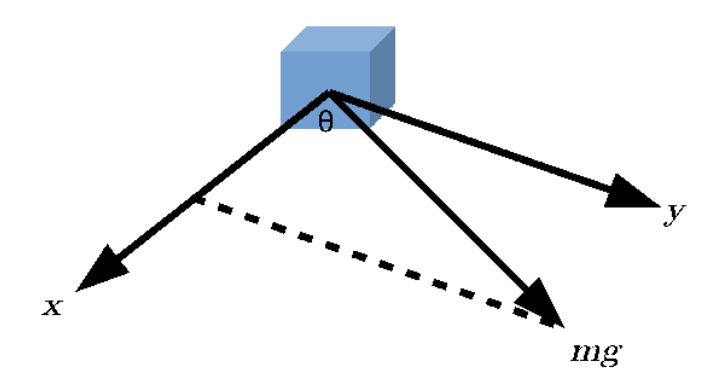
\includegraphics[width=0.5\textwidth]{gambar/gaya.png}
\end{figure}
\begin{choices}
\choice $mg\cos \theta \sin \theta$
\choice $mg\cos \theta \sin 2\theta$
\choice $mg\cos \theta \sin \theta$
\choice $mg$
\choice 0
\end{choices}

\textit{Jawaban: E}\\
Tidak ada komponen gaya pada arah $z$.

\vspace{0.5cm}
\question Manakah di antara materi di bawah ini yang BUKAN merupakan pengurai cahaya?
\begin{choices}
\choice kisi
\choice prisma
\choice titik air di udara
\choice filter
\choice CD/DVD
\end{choices}

\textit{Jawaban: D}\\
Filter berperan untuk mentransmisikan cahaya pada rentang energi tertentu saja, bukan menguraikan cahaya.

\vspace{0.5cm}
\question Mengapa mencari komet baik dilakukan dengan binokuler?
\begin{choices}
\choice Komet adalah sumber titik, dan binokuler memiliki medan pandang sempit.
\choice Komet adalah sumber membentang, dan binokuler memiliki medan pandang luas.
\choice Komet tampak hanya sekejap, dan binokuler memiliki medan pandang sempit.
\choice Komet adalah sumber membentang, dan binokuler memiliki magnifikasi tinggi.
\choice Komet tampak lama di langit, dan binokuler memiliki magnifikasi tinggi.
\end{choices}

\textit{Jawaban: B}\\
Komet merupakan objek membentang sehingga dibutuhkan medan pandang yang cukup luas untuk dapat melihat bagian besar/keseluruhan komet. Komet dilangit berjalan cukup lambat, dapat terlihat dalam rentang beberapa hari.

\vspace{0.5cm}
\question Gambar di bawah menunjukkan spektrum awan debu di sekitar bintang (\textit{circumstellar dust}). Taksiran terbaik untuk temperatur awan debu tersebut adalah
\begin{figure}[H]
\centering
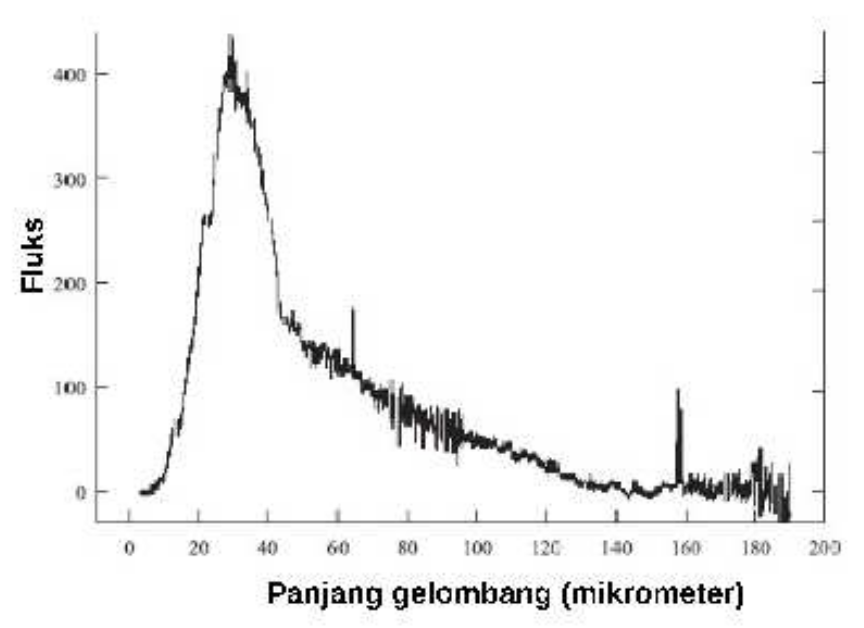
\includegraphics[width=0.5\textwidth]{gambar/spektrum.png}
\end{figure}
\begin{choices}
\choice 120 Kelvin
\choice 60 Kelvin
\choice 40 Kelvin
\choice 20 Kelvin
\choice 10 Kelvin
\end{choices}

\textit{Jawaban: A}\\
Tren profil spektrum mewakili kurva Planck suatu objek dengan temperatur efektif tertentu. Puncak fluks bersesuaian dengan energi pada panjang gelombang sekitar $\lambda_{\text{max}}=$ 25 mikrometer = 0,000025 m (hati-hati banyak garis emisi). 

Dengan memanfaatkan Hukum Wien
\begin{eqnarray*}
T_{\text{eff}}&=&\frac{0,002898}{\lambda_{\text{max}}}\\
T_{\text{eff}}&=&\frac{0,002989}{0,000025}=115,92\\
&\approx& 120 \quad \text{Kelvin}
\end{eqnarray*}


\vspace{0.5cm}
\question Para astronom meyakini bahwa \textit{exoplanet} serupa Bumi yang mungkin mengemban kehidupan dapat dicari jika peralatan interferometer ditempatkan di angkasa luar. Jika hal itu terjadi, empat garis serapan dalam panjang gelombang kasatmata dan inframerah dapat dideteksi dalam spektrum \textit{exoplanet}, dengan kemungkinan karakteristik sebagai berikut:
\begin{enumerate}[I.]
\item Terdapat pita serapan Ozon (O$_3$) dalam spektrum yang memperlihatkan kelimpahan oksigen, yang mungkin dihasilkan oleh jasad kehidupan.
\item Profil spektrum, yang menandakan temperatur \textit{exoplanet}, sesuai dengan syarat agar air berada dalam fase cair.
\item Terdapat pita serapan CO$_2$ yang sangat kuat dan menunjukkan keberadaan atmosfer.
\item Terdapat tanda-tanda serapan H$_2$O di berbagai rentang spektrum yang menunjukkan kelimpahan air yang besar sebagai pertanda keberadaan lautan.
\end{enumerate}
Urutan prioritas keutamaan indikator-indikator di atas, yang diacu orang saat ini, bagi pencarian \textit{exoplanet} serupa Bumi adalah:
\begin{choices}
\choice I-II-III-IV
\choice II-I-IV-III
\choice II-III-I-IV
\choice IV-I-III-II
\choice III-II-IV-I
\end{choices}

\textit{Jawaban: C}\\
Urutan berdasarkan prioritas pencarian, dari yang umum ke khusus atau dari yang mudah ke yang lebih susah.

\begin{tabular}{l c l}
II &:& Apakah temperaturnya menunjang air dalam wujud cair? \\
   & & Cukup dari profil spektrum (mencari puncaknya; hukum Wien),\\
   & & untuk mencari apakah berpeluang ``ada'' air dalam bentuk cair \\
   & & (belum sampai tahap kelimpahan/jumlah air).\\
III&:& Apakah planetnya memiliki atmosfer? \\
   & & Dari pita serapan CO$_{2}$ yang biasanya melimpah di planet kebumian,\\
   & & tanpa atmosfer kehidupan akan susah terbentuk, bombardir partikel dan \\
   & & radiasi akan sampai ke permukaan planet tanpa adanya atmosfer.\\
I  &:& Apakah ada oksigen? Dari pita serapan Ozon (O$_3$).\\
IV &:& Apakah ada lautan? Berapa jumlah air dalam bentuk cair atau gas?\\
   & & Dari serapan H$_{2}$O di berbagai rentang spektrum.
\end{tabular}



\vspace{0.5cm}
\question Kalender Cina merupakan sistem lunisolar di mana setiap hari libur Imlek bertepatan dengan konjungsi Bulan dengan menggunakan waktu UT+8 jam. Dalam kalender nasional, tanggal 19 Februari 2015 merupakan hari libur tahun baru Imlek 2566, dan konjungsi Bulan terjadi pada tanggal 19 Februari 2015 jam 07:48 WITA. Hari libur Imlek lainnya, hari libur tahun baru Imlek 2565 bertepatan dengan 31 Januari 2014 dan hari libur Imlek 2564 bertepatan dengan 10 Februari 2013. Satu tahun kalender Cina terdiri dari 354 hari, 355 hari, 384 hari, atau 385 hari. Dengan demikian, dalam rentang tahun baru Imlek 2551 dan tahun baru Imlek 2570, jumlah tahun baru Imlek dengan jumlah hari 384 atau 385 hari adalah
\begin{choices}
\choice 2
\choice 5
\choice 7
\choice 9
\choice 10
\end{choices}

\textit{Jawaban: C}
\begin{itemize}
\item Kalender Cina adalah kalender lunisolar yang awal tahunnya (tahun baru) ditentukan berdasarkan hari yang merupakan ``bulan baru kedua setelah \textit{winter solstice}'', sehingga tahun baru Cina hanya mungkin terjadi antara 21 Januari hingga 20 Februari. Kalender lunisolar merupakan kalender yang menggabungkan fenomena revolusi Bumi mengelilingi Matahari dan revolusi Bulan mengelilingi Bumi. 

\item Dalam satu tahun tropis, Bulan akan mengalami 12,37 kali periode sinodis (bulan baru kembali ke bulan baru). Hal ini menyebabkan
\begin{itemize}
\item Tahun hijriah selalu maju $\sim 11$ hari terhadap kalender masehi.
\item Satu tahun dalam kalender lunisolar bisa berjumlah 12 bulan (basit) atau 13 bulan (kabisat). Contoh kalender lunisolar: Hebrew (Yahudi), Buddhist, Hindu, Kurdish, Bengali, Tibet, Chinese, Japanese, Vietnamese, Mongolian, Korean calendars, Babylonian, dll.
\item dlsb
\end{itemize}

\item Meton ($\sim$ 440 BC) mendapati bahwa 235 kali periode sinodis Bulan hampir bertepatan dengan 19 tahun tropis. Hal ini menyebabkan siklus 19 tahun merupakan siklus yang paling banyak digunakan dalam kalender lunisolar.
\begin{eqnarray*}
19 \quad \text{tahun} &=& 19 \cdot \frac{365,2422}{29,5306}\\
&=& 234,997 \quad \text{periode sinodis bulan.}
\end{eqnarray*}
Dalam 19 tahun dibutuhkan $235 - (19 \times 12) = 7$ bulan tambahan untuk menyinkronkan siklus. Tambahan ini (berupa bulan ke-13) biasa ditambahkan pada tahun-tahun berikut: 3, 5, 8, 11, 13, 16, dan 19, dalam satu siklus 19 tahunan yang kemudian disebut siklus \textit{Metonic}.

\item Dalam rentang 2551 sampai 2570 (19 tahun) berapa jumlah tahun yang panjangnya 384 atau 385 hari? $\rightarrow 7$ \smiley 

\item Cara sederhana lain bisa dilakukan, setiap tahun kita tahu kalender lunar (contoh: hijriah) bergeser setiap $365-354 = 11$ hari, maka selisih hari ini akan melebihi satu periode sinodis Bulan setiap $\frac{30}{11} = 2,7 \approx 3$ kali. Setiap 2 sampai 3 tahun, kalender lunisolar harus digeser $\rightarrow$ ditambah 1 bulan sehingga panjangnya menjadi 384 hari. Oleh sebab itu, dalam $2570-2551 = 19$ tahun akan ada tahun yang lamanya 13 bulan tersebut sejumlah $\frac{19}{2,7} = 7$ kali \smiley
\end{itemize}


\vspace{0.5cm}
\question Jika pengamat di kota Bandung (lintang geografis $-6\degree57'$ LS dan bujur geografis $107\degree34'$ BT) mengamati Matahari terbenam pada tanggal 21 Juni pukul 17:43 WIB, maka pengamat di Manado (lintang geografis $+1\degree29'$ LU dan bujur geografis $124\degree52'$ BT) akan mengamati Matahari terbenam di tanggal yang sama pada pukul
\begin{choices}
\choice 16:13 WIB
\choice 16:25 WIB
\choice 16:48 WIB
\choice 17:07 WIB
\choice 17:13 WIB
\end{choices}

\textit{Jawaban: C}\\
Rumus umum untuk mencari sudut jam ($HA$) suatu benda yang tenggelam, diamati seseorang di lintang tertentu, dapat diturunkan dari segitiga bola $KLU - Z - \text{objek}$ (lihat gambar di bawah).

Rumus \textit{cosinus} pada segitiga bola
$$\cos a = \cos b \cos c + \sin b \sin c \cos A$$
dapat diterapkan pada segitiga ini
\begin{eqnarray*}
\cos 90\degree &=& \cos{(90\degree - \phi)} \cos{(90\degree - \delta)} + \sin{(90\degree - \phi)} \sin{(90\degree - \delta)} \cos HA\\
0 &=& \sin{\phi} \sin{\delta} + \cos{\phi}\cos{\delta}\cos{HA}\\
\cos{HA} &=& - \frac{\sin{\phi} \sin{\delta}}{\cos{\phi}\cos{\delta}}\\
\cos{HA} &=& -\tan{\phi} \tan{\delta}
\end{eqnarray*}

\begin{figure}[H]
\centering
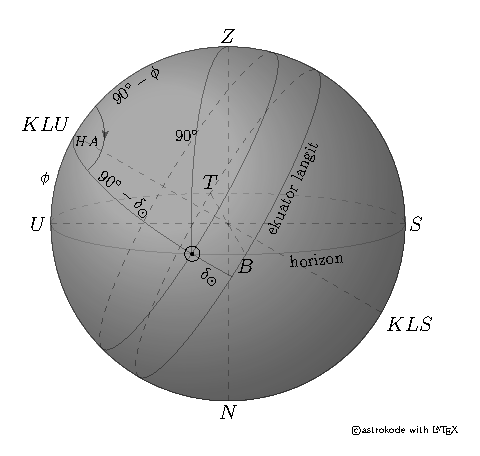
\includegraphics[width=0.7\textwidth]{gambar/sunset.pdf}
\end{figure}

Pada tanggal 21 Juni $\delta_{\odot} = 23,5\degree$.

Di Bandung ($\phi_B = -6,95\degree$; $\lambda_B = 107,57\degree$ BT), $HA$ Matahari ketika tenggelam adalah 
\begin{eqnarray*}
\cos HA_{B} &=& - \tan \phi_{B} \tan \delta_{\odot} \\
HA_B &=& 86,9617\degree = 5^j 48^m
\end{eqnarray*}
Jika Matahari tenggelam pukul 17:43 WIB, maka ia berada di kulminasi atas pada pukul 11:55 $^\star$. Di Manado ($\phi_M = +1,483\degree$; $\lambda_M = 124,87\degree$ BT) Matahari akan di kulminasi atas pada pukul 
\begin{eqnarray*}
\text{11:55 WIB} - \left( \frac{124,87\degree - 107,57\degree}{15\degree} \right) = \text{11:55 WIB} - 1^j 9^m = \text{10:46 WIB}
\end{eqnarray*}

Di Manado, $HA$ Matahari ketika tenggelam adalah
\begin{eqnarray*}
\cos HA_{M} &=& - \tan \phi_{M} \tan \delta_{\odot} \\
HA_M &=& 90,645\degree = 6^j 2^m 35^d
\end{eqnarray*}
bertepatan dengan pukul 10:46 WIB + $6^j 2^m 35^d$ = 16:48 WIB.

Catatan:\\
$^\star$ Ketika Matahari berada di kulminasi atas bisa saja tidak tepat dengan jam 12:00 waktu lokal dikarenakan orbit elips dari Bumi. Kecepatan orbit Matahari di langit berubah karena kecepatan revolusi Bumi yang berubah. Selisih antara $HA$ Matahari sebenarnya dan $HA$ Matahari rata-rata (\textit{mean solar}) disebut \textit{equation of time} ($\xi$).
\begin{equation*}
\xi = HA_{\odot} - HA_{MS}
\end{equation*}


\vspace{0.5cm}
\question Kelompok siswa di Yogyakarta (BT 110,24; LS 7,48) merencanakan mengamati \textit{Milky Way}. Kelompok siswa tersebut memperoleh informasi posisi koordinat ekuatorial (saat pengamatan) asensiorekta dan deklinasi arah pusat Galaksi $17^h45^m37,224^s$ dan $-28\degree56'10,23''$. Bila pengamatan dilakukan malam hari tanggal 20 Mei maka diharapkan kelompok siswa tersebut akan mengamati pusat Galaksi berkulminasi atas pada jam
\begin{choices}
\choice 1 jam 37 m setelah jam 24:00 WIB
\choice 1 jam 37 m sebelum jam 24:00 WIB
\choice tepat jam 24:00 WIB
\choice 2 jam 46 menit sebelum jam 24:00 WIB
\choice 2 jam 46 menit setelah jam 24:00 WIB
\end{choices}

\textit{Jawaban: A}\\
Pada tanggal 20 Mei, $RA_{\odot} \sim 4^h$.\\
Pusat galaksi yang berkulminasi atas artinya memiliki $HA_{G} = 0^{h}$.
\begin{eqnarray*}
LST = HA_{\odot} + RA_{\odot} &=& HA_{G} + RA_{G}\\
HA_{\odot} + 4^{h} &=& 0^{h} + 17^{h} 45^{m} 37,224^{s}\\
HA_{\odot} &=& 13^{h} 45^{m} 37,224^{s}
\end{eqnarray*}
Saat $HA_{\odot} = 13^{h} 45^{m} 37,224^{s}$, artinya waktu lokal di tempat tersebut adalah pukul $\sim$ 01:45.\\
Selisih dengan waktu sipil (\textit{zone time}/ \textit{civil time}) $= (110,24\degree - 105\degree)/15\degree = 0.34933^h = 21^m$.\\
Sehingga jam dinding di sana menunjukkan waktu 01:45 - $21^{m} \sim$ 01:24 WIB.  

\vspace{0.5cm}
\question Gerhana Matahari terjadi ketika piringan Bulan menutupi piringan Matahari. Misalkan piringan Bulan dan Matahari tampak dengan diameter sudut yang sama ($D$) dan kedua titik pusat piringan objek terpisah oleh jarak $D/2$. Dari gambar di bawah ini, berapakah rasio piringan Matahari yang tertutup piringan Bulan?
\begin{figure}[H]
\centering
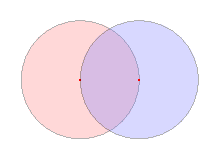
\includegraphics[width=0.3\textwidth]{gambar/duaLingkaran.pdf}
\end{figure}
\begin{choices}
\choice 0,3
\choice 0,4
\choice 0,5
\choice 0,6
\choice 0,7
\end{choices}

\textit{Jawaban: B} \\
\begin{figure}[H]
\centering
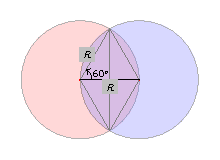
\includegraphics[width=0.4\textwidth]{gambar/duaLingkaran_jwb.pdf}
\end{figure}
Perhatikan gambar di atas, luas piringan Matahari yang tertutup oleh piringan bulan adalah luas 2 tembereng. 
\begin{eqnarray*}
L &=& 2 \cdot \text{Luas tembereng}\\
&=& 2 \cdot (\text{Luas juring} - \text{Luas segitiga})\\
&=& 2 \cdot \text{Luas juring} - 2 \cdot \text{Luas segitiga sama sisi}\\
&=& 2 \cdot \frac{1}{3} \pi R^{2} - 2 \cdot \left( \frac{1}{2} \cdot R \cdot \frac{1}{2} \sqrt{3} R \right) \\
&=& \frac{2}{3} \pi R^{2} - \frac{1}{2} \sqrt{3} R^{2} 
\end{eqnarray*}
Rasio terhadap luas piringan Matahari
\begin{eqnarray*}
\text{Rasio} &=& \frac{\frac{2}{3} \pi R^{2} - \frac{1}{2} \sqrt{3} R^{2}}{\pi R^{2}}\\
&=& \frac{2}{3} - \frac{\sqrt{3}}{2 \pi} = 0,391 \approx 0,4
\end{eqnarray*}

\vspace{0.5cm}
\question Pada jarak $d$, partikel angin Matahari memiliki kerapatan $\rho$ serta kecepatan $v$. Bila ketiga variabel tersebut diketahui, maka laju kehilangan massa Matahari (kg/detik) dapat dihitung dengan persamaan
\begin{choices}
\choice $\dot{M}=\rho v$
\choice $\dot{M}=2\pi d \rho v$
\choice $\dot{M}=4\pi d^2 \rho v$
\choice $\dot{M}=\frac{4\pi}{3}d^3 \rho$
\choice $\dot{M}=\frac{5\pi}{2}d^3 \rho v$
\end{choices}

\textit{Jawaban: C}\\
\begin{figure}[H]
\centering
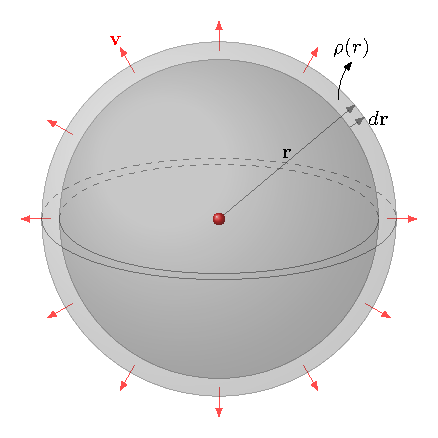
\includegraphics[width=0.4\textwidth]{gambar/solar_wind.pdf}
\end{figure}
Kita dapat mencari terlebih dahulu elemen massa angin Matahari yang berjalan $dM$. Pada jarak $r = d$ dari Matahari, besarnya elemen massa ini dapat digambarkan sebagai kulit bola dengan tebal $dr$ dan kerapatan $\rho(r)$.
\begin{eqnarray*}
dM &=& \rho(r) \cdot dV(r)\\
dM &=& \rho(r) \cdot 4 \pi r^{2} dr
\end{eqnarray*}
Elemen massa ini bergerak pada arah radial keluar dengan kecepatan $v$, sehingga laju kehilangan massa dapat ditulis menjadi
\begin{eqnarray*}
\frac{dM}{dt} &=& \frac{4 \pi r^2 \rho dr}{dt}\\
\frac{dM}{dt} &=& 4 \pi r^2 \rho \frac{dr}{dt}\\
\dot{M} &=& 4 \pi r^2 \rho v = 4 \pi d^2 \rho v 
\end{eqnarray*}
Cara sedikit putus asa, tetapi mungkin yang diminta oleh juri/pembuat soal:\\
Kita dapat mencari pilihan yang benar dengan analisis dimensi (di soal sudah diberikan petunjuk berupa satuan ``kg/s''), kebetulan hanya satu pilihan jawaban yang benar.

\vspace{0.5cm}
\question Sebuah koloni di Mars mengalami peningkatan populasi sehingga kebutuhan komunikasi jarak jauh mutlak dibutuhkan. Untuk itu, NASA meluncurkan satelit komunikasi stasioner terhadap Mars. Seperti satelit geostasioner, satelit tersebut memiliki periode orbit sama dengan periode rotasi planet Mars sehingga satelit berada pada bujur geografis yang tetap. Diukur dari pusat Mars, radius orbit satelit tersebut yang lebih dekat pada nilai yang benar adalah
\begin{choices}
\choice 16000 km
\choice 16600 km
\choice 18000 km
\choice 20000 km
\choice 22000 km
\end{choices}

\textit{Jawaban: D}\\
Massa Mars ($M$) $= 6,42 \times 10^{23}$ kg\\
Periode orbit satelit ``Mars-stasioner'' = periode rotasi Mars ($T$) = $24^j 37^m 22^{d},6$\\
Menggunakan hukum Kepler III
\begin{eqnarray*}
\frac{a^3}{T^2} &=& \frac{GM}{4 \pi^{2}} \\
a &=& \sqrt[3]{\frac{GMT^2}{4 \pi^{2}}} \\
a &=& \sqrt[3]{\frac{6,67 \times 10^{-11} \cdot 6,42 \times 10^{23} \cdot 88642,6^2}{4 \pi^{2}}}\\
a &=& 20426566,2 \quad \text{m} \\
a &=& 204265,66 \approx 20000 \quad \text{km} 
\end{eqnarray*}


\vspace{1cm}
\textbf{Soal Pilihan Ganda Bersyarat}\\
Untuk dua soal berikut ini, jawablah\\
A. jika 1, 2, dan 3 benar\\
B. jika 1 dan 3 benar\\
C. jika 2 dan 4 benar\\
D. jika 4 saja benar\\
E. jika semua benar\\

\question Pilihlah pernyataan yang benar.
\begin{enumerate}
\item Semakin tinggi temperatur suatu planet, maka semakin mudah planet tersebut kehilangan atmosfer.
\item Atmosfer planet dalam tersusun atas partikel yang relatif lebih ringan dibandingkan dengan atmosfer planet luar.
\item Planet luar dapat mempertahankan atmosfernya karena massanya yang besar dan jaraknya yang jauh dari Matahari.
\item Semakin besar planet, semakin mudah planet tersebut kehilangan atmosfer.
\end{enumerate}

\textit{Jawaban: B}\\
Penjelasan untuk masing-masing pernyataan:
\begin{enumerate}
\item Temperatur tinggi meningkatkan energi kinetik partikel penyusun atmosfer planet, sehingga partikel-partikel tersebut lebih mudah membebaskan diri dari ikatan gravitasi planet. (Pernyataan 1 BENAR)
\item Paparan radiasi memberi tambahan energi kinetik pada partikel penyusun atmosfer. Atmosfer planet dalam terpapar energi lebih tinggi daripada planet luar. Paparan energi itu dikonversi menjadi energi kinetik: $\frac{1}{2}mv^2$. Partikel bermassa kecil mendapat laju $v$ lebih besar sehingga lebih mudah lepas dari planet. Dengan demikian, partikel-partikel bermassa beratlah yang dapat bertahan terikat oleh planet dalam. (Pernyataan 2 SALAH)
\item Semakin jauh jarak planet dari Matahari semakin rendah fluks radiasi yang diterima (temperatur rendah), sehingga energi kinetik partikel penyusun atmosfer relatif rendah. Massa besar artinya gravitasi kuat sehingga kemampuan mengikat atmosfer tinggi. (Pernyataan 3 BENAR)
\item Makin besar planet, gravitasi makin kuat, atmosfer makin sulit lepas. (Pernyataan 4 SALAH)
\end{enumerate}

\vspace{0.5cm}
\question Di antara pernyataan di bawah ini, manakah yang BENAR?
\begin{enumerate}
\item Unsur yang lebih berat dari besi (Fe) dihasilkan saat ledakan Supernova.
\item Bintang deret utama melawan pengerutan gravitasi dengan tekanan elektron terdegenerasi. 
\item Bintang dengan massa yang cukup besar mampu melakukan reaksi fusi di inti yang menghasilkan unsur yang lebih berat dari besi (Fe).
\item Pada reaksi fusi hidrogen, empat inti hidrogen membentuk satu inti helium.  Total massa satu inti helium lebih kecil daripada total massa empat inti hidrogen.
\end{enumerate}

\textit{Jawaban: Tidak ada}\\
Penjelasan untuk masing-masing pernyataan:
\begin{enumerate}
\item Inti atom paling berat yang dapat dibentuk melalui nukleosintesis di pusat bintang yakni inti besi (Fe). Pembentukan inti lebih berat dari besi salah satunya melibatkan proses penangkapan neutron dalam proses cepat (\textit{r-process}/\textit{rapid process}). Proses ini terjadi ketika supernova. Saat supernova terjadi, banyak neutron bebas muncul sebagai pecahan dari inti-inti atom (karena energi tinggi, inti atom bisa pecah). Lingkungan supernova sangat rapat sehingga neutron-neutron yang bertebaran dapat segera ditangkap oleh inti atom, sebelum neutron-neutron tersebut meluruh. Dengan demikian, dapat dinyatakan bahwa supernova merupakan salah satu proses yang dapat menghasilkan inti-inti atom yang lebih berat daripada besi. (Pernyataan 1 BENAR)
\item Bintang deret utama melawan pengerutan gravitasi dengan tekanan gas dan tekanan radiasi. (Pernyataan 2 SALAH)
\item Nukleosintesis di pusat bintang tidak mampu menghasilkan inti atom lebih berat dari besi (Fe). (Pernyataan 3 SALAH)
\item Pembentukan satu inti Helium memerlukan empat inti Hidrogen melalui reaksi fusi. Massa satu inti Helium kurang dari total massa empat inti Hidrogen pembentuknya. Selisih massa $\Delta m$ ini yang dinamakan \textit{mass defect}, yang mewakili energi yang dilepas ketika inti baru terbentuk, sebesar $E=\Delta m c^2$. (Pernyataan 4 BENAR)
\end{enumerate}

\vspace{1cm}
\textbf{Soal Pilihan Ganda Sebab-Akibat}\\
Gunakan petunjuk ini untuk menjawab soal-soal berikut:
A. Pernyataan pertama dan kedua benar serta memiliki hubungan sebab-akibat.\\
B. Pernyataan pertama dan kedua benar, tetapi tidak memiliki hubungan sebab-akibat.\\
C. Pernyataan pertama benar, sedangkan pernyataan kedua salah.\\
D. Pernyataan pertama salah, sedangkan pernyataan kedua benar\\
E. Kedua pernyataan salah.\\

\question Hasil penelitian astronom pada tahun 1998 tentang energi gelap menunjukkan bahwa alam semesta kita sekarang sedang mengalami pengembangan yang diperlambat.
\begin{center}
SEBAB
\end{center}
\noindent Gaya gravitasi yang selalu bersifat tarik menarik paling mendominasi dalam skala besar.

\textit{Jawaban: E}\\
Hasil penelitian astronom pada tahun 1998 tentang energi gelap menunjukkan bahwa alam semesta kita sekarang sedang mengalami pengembangan yang \textit{dipercepat}. (Pernyataan pertama SALAH)\\
Pada skala besar, energi gelap (\textit{dark energy}) mendominasi, menyebabkan alam semesta mengembang dipercepat. (Pernyataan kedua SALAH)

\vspace{0.5cm}
\question Materi antar bintang membuat nilai magnitudo bintang yang kita lihat mengecil.
\begin{center}
SEBAB
\end{center}
\noindent Partikel materi antar bintang menyerap cahaya bintang yang berada di belakangnya.

\textit{Jawaban: D}\\
Materi antar bintang membuat kecerlangan bintang yang kita lihat mengecil, nilai magnitudo membesar. (Pernyataan pertama SALAH)\\
Partikel materi antar bintang menyerap cahaya bintang yang berada di belakangnya. (Pernyataan kedua BENAR)


%%%%%%%%%%%%%%%%%%%%%%%%%%%%%%%%%%%%%%%%%%
\vspace{1cm}
\textbf{Soal Essay Pendek}

\question Diketahui diameter pupil mata adalah 5 mm. Dengan menggunakan kriteria Rayleigh,
\begin{enumerate}[(a)]
\item hitunglah limit resolusi sudut mata manusia pada panjang gelombang 550 nm,
\item hitunglah perbandingan jawabanmu ini dengan diameter sudut Bulan dan planet Jupiter (saat oposisi).
\item Jelaskan, apakah mata telanjang kita mampu memisahkan ciri-ciri pada piringan Bulan dan piringan Jupiter?
\end{enumerate}

\textit{Jawaban:}
\begin{enumerate}[(a)]
\item Sudut terkecil yang masih dapat dipisahkan (limit resolusi sudut):
\begin{equation*}
\theta_{res} = \frac{1,22 \lambda}{D} \qquad (rad)
\end{equation*}
untuk mata manusia
\begin{eqnarray*}
\theta_{res} = \frac{1,22 \cdot 550 \times 10^{-6}}{5} &=& 1,342 \times 10^{-4} \quad rad\\
&=& 27,68''
\end{eqnarray*}

\item Diameter sudut
\begin{figure}[H]
\centering
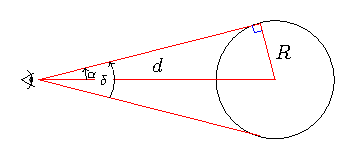
\includegraphics[width=0.49\textwidth]{gambar/diametersudut_umum.pdf}
\end{figure}
\begin{minipage}[t]{0.5\textwidth}
Bulan
\begin{eqnarray*}
\sin \alpha_{\leftmoon} &=& \frac{R_{\leftmoon}}{d_{\oplus \leftmoon}} = \frac{1738}{384399}\\
\alpha_{\leftmoon} &=& 0,259\degree\\
\delta_{\leftmoon} &=& 0,518\degree = 1865,2''\\
\frac{\theta_{res}}{\delta_{\leftmoon}} &=& 0,01484
\end{eqnarray*}
\end{minipage}
\begin{minipage}[t]{0.5\textwidth}
Jupiter saat oposisi, 

jaraknya dari Bumi adalah $d_{\oplus \jupiter} = d_{\odot \jupiter} - d_{\odot \oplus}$  
\begin{eqnarray*}
\sin \alpha_{\jupiter} &=& \frac{R_{\jupiter}}{d_{\oplus \jupiter}} = \frac{71492}{6,2873 \times 10^{8}}\\
\alpha_{\jupiter} &=& 6,515 \times 10^{-3} ~^{\circ}\\
\delta_{\jupiter} &=& 0,013\degree = 46,9''\\
\frac{\theta_{res}}{\delta_{\jupiter}} &=& 0,59
\end{eqnarray*}
\end{minipage}

Cara lain menghitung diameter sudut (saat $d \ggg D$):
\begin{figure}[H]
\centering
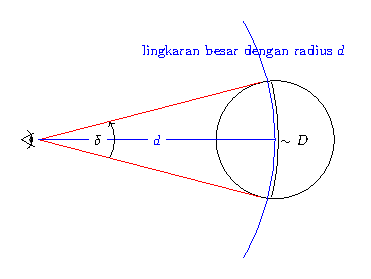
\includegraphics[width=0.5\textwidth]{gambar/diametersudut_rad.pdf}
\end{figure}

\begin{eqnarray*}
\delta &=& \frac{D}{d} \quad (rad)\\
\delta &=& \frac{206265 \cdot D}{d} \quad ('')
\end{eqnarray*}
dengan $D$ adalah diameter objek dan $d$ adalah jarak dari pengamat ke objek.

\item Diameter sudut kedua objek lebih besar dari limit sudut resolusi, sehingga keduanya akan tampak sebagai piringan atau \textit{extended object}. Untuk dapat memisahkan ciri-ciri/\textit{feature} dari piringan kedua objek, semisal kawah di Bulan atau bintik merah di Jupiter, maka haruslah diameter sudut dari \textit{feature} tersebut lebih besar dari limit sudut resolusi mata. 
\end{enumerate}


\vspace{0.5cm}
\question Dari hasil astrofotografi, diketahui ukuran Nebula Kepiting (M1) adalah 6'. Objek tersebut berada pada jarak 100 pc. Dari hasil pengukuran efek Doppler, kecepatan pengembangan nebula diketahui sebesar 1400 km/detik. Anggaplah usia Nebula Kepiting pada waktu tertentu adalah waktu yang diperlukan untuk Nebula Kepiting dari sebuah titik hingga mencapai ukuran pada waktu itu.
\begin{enumerate}[(a)]
\item Hitunglah radius linear Nebula Kepiting!
\item Hitung pula usia Nebula Kepiting!
\end{enumerate}

\textit{Jawaban:}
\begin{enumerate}[(a)]
\item Identik dengan soal sebelumnya, radius linier M1 dapat ditentukan dari ukuran bentangan di langit dan jaraknya.
\begin{eqnarray*}
D &=& \delta \cdot d\\
&=& 1,74533 \times 10^{-3} \text{(rad)} \cdot 100 \text{(pc)}\\
&=& 0,17453 \quad \text{pc}\\
R &=& 0,08726 \quad \text{pc} \quad = \quad 2,6926 \times 10^{12} \quad \text{km} 
\end{eqnarray*}

\item Usia ``ledakan'' nebula Kepiting dapat ditentukan dari ukuran sekarang dan kecepatan pengembangannya. Dengan menganggap tidak ada perubahan kecepatan pengembangan, ukuran bintang sebelum meledak jauh lebih kecil dari ukuran nebula (dianggap titik), serta ledakannya adalah simetri bola, maka
\begin{eqnarray*}
t &=& \frac{R}{v}\\
  &=& \frac{2,6926 \times 10^{12}}{1400}\\
  &=& 1,92327 \times 10^{9} \quad \text{detik} \\
  &=& 60,945 \quad \text{tahun}
\end{eqnarray*}
\end{enumerate}


\vspace{0.5cm}
\question Sebuah teleskop digunakan untuk melihat Bulan yang memiliki diameter sudut 30 menit busur. Medan pandang teleskop sama dengan diameter sudut Bulan dan teleskop tidak dilengkapi motor. Dalam waktu berapa lamakah Bulan sepenuhnya akan hilang dari medan pandang teleskop?

\textit{Jawaban:}

Saat digunakan untuk melihat Bulan, diasumsikan Bulan sepusat dengan medan pandang teleskop. Jika teleskop tidak \textit{tracking} atau bergerak mengikuti langit, maka Bulan perlahan-lahan akan menghilang dari medan pandang teleskop disebabkan gerak semunya di langit. Gerak semu Bulan di langit diakibatkan oleh rotasi Bumi (gerak semu harian) dan revolusi Bulan.

Diameter sudut Bulan $= 30' = 0,5\degree$

Kecepatan sudut Bulan di langit
\begin{eqnarray*}
\omega_{relatif} &=& \omega_{rotasi} - \omega_{rev \leftmoon}\\
&=& \frac{360\degree}{23^j56^m4^d} - \frac{360\degree}{27,3217^{hari}}\\
&=& 4,178 \times 10^{-3} ~\degree / detik - 1,525 \times 10^{-4} ~\degree / detik\\
&=& 4,0255 \times 10^{-3}  ~\degree / detik
\end{eqnarray*}
dengan asumsi Bulan berada di ekuator langit (deklinasi nol), maka waktu yang diperlukan oleh Bulan untuk bergeser dari tengah medan pandang sampai seluruh piringannya hilang adalah
\begin{eqnarray*}
t &=& \frac{0,5 \degree}{4,0255 \times 10^{-3}  ~\degree / detik}\\
&=& 124,2 \quad \text{detik}.
\end{eqnarray*}
Catatan: 
\begin{itemize}
\item Jika yang ditanyakan adalah waktu maksimum Bulan berada di dalam medan pandang teleskop, maka butuh waktu 248,4 detik (Bulan mulai masuk medan pandang hingga keluar).
\item Jika deklinasi Bulan tidak nol, maka durasinya dapat lebih lama.
\end{itemize}


\vspace{0.5cm}
\question Analisis spektrum bintang ganda spektroskopik bergaris ganda yang juga merupakan bintang ganda gerhana dengan periode orbit $P=8,6$ tahun menunjukkan pergeseran Doppler maksimum dari garis Balmer hidrogen H$_{\alpha}$ (656,281 nm), untuk komponen sekunder adalah $\lambda_s=0,072$ nm dan untuk komponen primer $\lambda_p=0,0068$ nm. Adapun bentuk kurva kecepatan radialnya adalah sinusoidal. Hitunglah setengah sumbu panjang sistem bintang ganda ini dinyatakan dalam satuan astronomi (au)!

\textit{Jawaban:}

Dapat diasumsikan bahwa inklinasi orbit bintang ganda $\sim 90\degree$ (``bintang ganda gerhana'') dan orbit lingkaran (``sinusoidal''). Sehingga, dari pengamatan spektrumnya dapat langsung diperoleh kecepatan orbit masing-masing bintang terhadap pusat massa (karena merupakan kecepatan radial maksimum).

Menggunakan Efek Doppler
\begin{equation*}
\frac{\Delta \lambda}{ \lambda_{0}} = \frac{v_{radial}}{c}
\end{equation*}
diperoleh
\begin{equation*}
v_{1} = \frac{0,0068}{656,281} \cdot 3 \times 10^{5} = 3,1 \quad \text{km/s} \qquad \text{dan} \qquad v_{2} = \frac{0,072}{656,281} \cdot 3 \times 10^{5} = 32,9 \quad \text{km/s}
\end{equation*}

Kecepatan untuk orbit lingkaran adalah
\begin{equation*}
v = \frac{2 \pi r}{P},
\end{equation*}
sehingga,
\begin{eqnarray*}
a &=& r_{1} + r_{2} \\
&=& \frac{v_1 P}{2 \pi} + \frac{v_2 P}{2 \pi} = 1,339 \times 10^{8} + 1,421 \times 10^{9}\\
&=& 1,555 \times 10^{9} \quad \text{km}\\
&=& 10,39 \quad \text{au}
\end{eqnarray*}


\vspace{0.5cm}
\question Perhatikanlah sebuah teropong yang menemukan sebuah protogalaksi pada \textit{redshift} $z=12$ misalnya teropong yang dimiliki Yale University di Kitt Peak berdiameter 3,5 meter (optikal). Cahaya dari protogalaksi memuat garis emisi H$_{\alpha}$ (semacam \textit{tracer} dari laju pembentukan bintang). Panjang gelombang yang tertinggal dari garis H$_{\alpha}$ adalah 0,656 mikron di bagian optikal merah pada spektrumnya.
\begin{enumerate}[(a)]
\item Untuk protogalaksi ini, berapakah panjang gelombang H$_{\alpha}$ yang teramati?
\item Jika teropong mampu mengamati gelombang dalam rentang 0,3-2,2 mikron, dapatkah sebuah teropong inframerah-optikal di permukaan Bumi (semacam teropong yang disebutkan dalam soal) mengamati garis H$_{\alpha}$?
\item Carilah kerapatan rata-rata dari materi yang berkaitan dengan $z=12$. Di sini diambil asumsi bahwa dalam alam semesta saat (hari) ini memiliki kerapatan materi sebesar $2,4\times 10^{-27}$ kgm$^{-3}$.
\end{enumerate}

\textit{Jawaban:}
\begin{enumerate}[(a)]
\item Notasi $z$ untuk \textit{redshift} sering digunakan dalam kosmologi, dengan
\begin{eqnarray*}
z &=& \frac{\Delta \lambda}{\lambda_{0}} = \frac{\lambda - \lambda_{0}}{\lambda_{0}}\\
\lambda &=& \lambda_{0} (z + 1)\\
 \lambda &=& 8,528 \quad \text{mikron}
\end{eqnarray*}

\item Tidak bisa karena panjang gelombang yang teramati ($\lambda$) berada di luar rentang kemampuan teleskop.

\item Dalam kosmologi terdapat faktor skala $a(t)$ yang didefinisikan sebagai 
\begin{equation*}
r(t) = a(t) r_{0}
\end{equation*}
dengan $r(t)$ dan $a(t)$ adalah jarak antar dua titik (\textit{proper distance}) dan faktor skala saat $t$, sedangkan $r_{0}$ adalah jarak antar dua titik tersebut saat $t_0$ (sekarang), sehingga menurut definisi ini $a(t_0) = 1$.
Hubungan \textit{redshift} ($z$) dan faktor skala ($a$) adalah
\begin{equation*}
1 + z(t_{obs}) = \frac{a(t_{obs})}{a(t_{em})}
\end{equation*}
Pengamat ada dalam epoch alam semesta saat ini ($t_{obs} = t_0$), sehingga $a(t_{obs}) = 1$.
\begin{equation*}
1 + z = \frac{1}{a}
\end{equation*}
Semakin besar ukuran alam semesta, semakin kecil kerapatan materi (total ``massa''nya tetap). Kerapatan materi alam semesta akan berbanding terbalik dengan pangkat tiga faktor skala
\begin{equation*}
\rho \sim \frac{1}{a^3},
\end{equation*}
sehingga,
\begin{eqnarray*}
\rho &\sim& (1 + z)^{3}\\
\frac{\rho}{\rho_0} &=& \left(\frac{1+z}{1+z_0}\right)^{3} = \left(\frac{1+z}{1}\right)^{3}\\
\rho &=& \rho_0 (1+z)^3 = 5,273 \times 10^{-24} \quad \text{kg/m}^3
\end{eqnarray*}
\end{enumerate}


\vspace{0.5cm}
\question Salah satu metode penentuan jarak galaksi spiral adalah relasi Tully-Fisher yakni luminositas sebanding dengan kecepatan rotasi maksimum pangkat empat. Diamati sebuah galaksi spiral $A$ (yang mirip dengan Bimasakti) dengan radius 30 kpc dan memiliki 200 milyar bintang serupa Matahari. Diperoleh magnitudo galaksi tersebut adalah $m_B=11$ dan kecepatan rotasi maksimum sebesar 250 km/detik. Jika kecepatan rotasi maksimum Bimasakti sebesar 220 km/detik, maka
\begin{enumerate}[(a)]
\item berapakah jarak galaksi $A$ tersebut?
\item Berapakah diameter sudut galaksi $A$ tersebut?
\item Taksirlah berapa magnitudo Bimasakti jika dilihat dari galaksi $A$!
\end{enumerate}

\textit{Jawaban:}
\begin{enumerate}[(a)]
\item Asumsi semua bintang di galaksi A berkontribusi dalam kecerlangannya. Magnitudo mutlak bintang serupa Matahari ($M_B$) adalah 5,48 sehingga
\begin{eqnarray*}
M_{gal} - M &=& -2,5 \log \frac{200 \times 10^9 L_{\odot}}{L_{\odot}}\\
M_{gal} &=& -22,773,\\
\end{eqnarray*}
selanjutnya dengan asumsi tidak ada serapan,
\begin{eqnarray*}
m - M &=& -5 + 5 \log d\\
11 + 22,773 &=& -5 + 5 \log d\\
d &=& 56,822 \quad \text{Mpc}
\end{eqnarray*}

\item Diameter sudut galaksi dapat ditentukan
\begin{eqnarray*}
\delta &=& \frac{D}{d}\\
&=& \frac{60}{56822} \\
&=& 1,056 \times 10^{-3} \quad \text{rad}\\
&=& 3,63 \quad \text{menit busur}
\end{eqnarray*}

\item Karena jaraknya sama, maka
\begin{eqnarray*} 
m_{\text{Bima Sakti}} - m_{\text{gal A}} = -2,5 \log \frac{L_{\text{Bima Sakti}}}{L_{\text{gal A}}}
\end{eqnarray*}
menggunakan metode Tully-Fisher
\begin{eqnarray*} 
m_{\text{Bima Sakti}} - m_{\text{gal A}} &=& -2,5 \log \left(\frac{v_{\text{Bima Sakti}}}{v_{\text{gal A}}}\right)^{4}\\
m_{\text{Bima Sakti}} - 11 &=& -2,5 \log \left( \frac{220}{250} \right)^{4}\\
m_{\text{Bima Sakti}} &=& 11,55
\end{eqnarray*}
Jadi magnitudo galaksi Bima Sakti di filter B  ($m_B$) = 11,55.
\end{enumerate}


\vspace{0.5cm}
\question Pada suatu saat, okultasi planet Jupiter oleh Bulan terjadi pada pukul 21:00 ketika ketinggian Jupiter $45\degree$ di atas horizon timur. Seorang pengamat di kota A tidak dapat melihat Jupiter tertutup penuh oleh Bulan di saat puncak okultasi. Melalui teropong, ia hanya melihat lingkaran Bulan bersinggungan luar dengan Jupiter. Sementara itu, pengamat di kota B melihat Jupiter tertutup penuh oleh piringan Bulan. Namun dalam waktu yang sangat singkat, Jupiter muncul kembali.
\begin{enumerate}[(a)]
\item Gambarkanlah geometri dari peristiwa itu!
\item Berapakah jarak antara kota A dan kota B?
\end{enumerate}

\textit{Jawaban:}

\begin{enumerate}[(a)]
\item Sketsa geometri peristiwa
\begin{figure}[H]
\centering
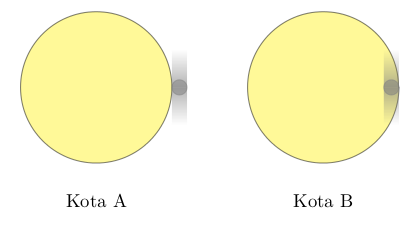
\includegraphics[width=0.5\textwidth]{gambar/moonJup.png}
\end{figure}
Dengan syarat: (1) kota A dan kota B melihat peristiwa ini bersamaan, (2) jalur Jupiter seperti di atas, geometri paling sederhana yang masih mungkin adalah sebagai berikut:
\begin{figure}[H]
\centering
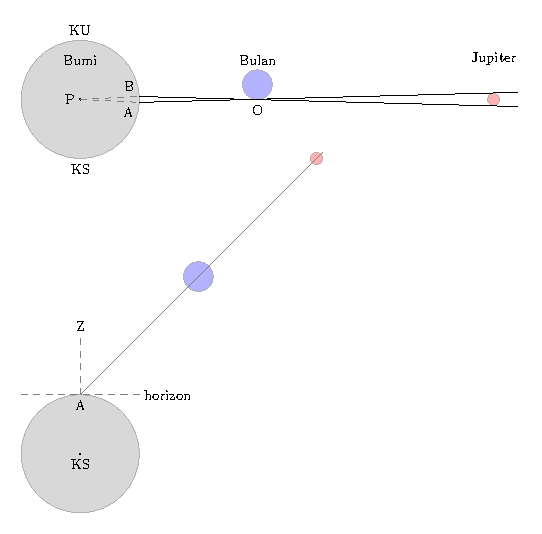
\includegraphics[width=0.7\textwidth]{gambar/moonJup2.pdf}
\end{figure}

\item Dari jam pengamatan (21:00) dan ketinggian ($45\degree$ di atas horizon timur) dapat diketahui bahwa Jupiter dan Bulan sedang dalam posisi ``dekat'' oposisi.

Diameter sudut Jupiter dilihat dari $O$ akan sama dengan $\angle AOB$. Jarak $O$ ke Jupiter ($J$) dapat diperkirakan karena Bulan dan Jupiter keduanya dalam posisi oposisi dari Matahari.
\begin{eqnarray*}
\angle AOB &=& \delta_J = \frac{D}{d_{OJ}}\\ 
&=& \frac{2 \cdot 71492}{7,7833 \times 10^{8} - 1,496 \times 10^{8} - 3,844 \times 10^{5}}\\
&=& 0,0002275563 \quad \text{rad}\\
&=& 0,013038 \degree
\end{eqnarray*}
dengan $D$ adalah diameter Jupiter.

Dengan asumsi sederhana bahwa $\triangle AOB$ adalah segitiga sama kaki, maka dapat di hitung $\angle APB$
\begin{eqnarray*}
AB &=& AB\\
R_{\oplus}^{2} + R_{\oplus}^{2} - 2R_{\oplus}^{2}\cos{\angle APB} &=& d^{2} + d^{2} - 2d^{2}\cos{\angle AOB} \\
2R_{\oplus}^{2} (1 - \cos \angle APB) &=& 2d^{2} (1 - \cos \angle AOB)\\
\cos \angle APB &=& 1 - \left(\frac{d}{R_{\oplus}}\right)^{2} (1 - \cos{\angle AOB})\\
\angle APB &=& 0,7858\degree
\end{eqnarray*}
dengan $d \approx d_{\oplus\leftmoon}$. Selanjutnya jarak A dan B dapat dicari dengan
\begin{eqnarray*}
\frac{0,7858\degree}{360\degree} \times 2 \pi 6378 = 87,47 \quad \text{km}
\end{eqnarray*}

Catatan:
\begin{itemize}
\item Lintasan Jupiter akan dekat dengan ekliptika langit.
\item Titik $O$ tidak berada dipermukaan Bulan; jarak $O$ ke Jupiter dan $O$ ke Bumi didekati seolah-olah $O$ adalah Bulan itu sendiri.
\item Jika $OA$ dan $OB$ tidak sama kaki, maka perhitungan menjadi lebih rumit karena harus memasukkan faktor \textit{paralaks horizon} (berpengaruh besar pada penentuan jarak kota A dan B).
\end{itemize}

\end{enumerate}

\end{questions}


\newpage
\center \LARGE \textbf{Daftar Konstanta}

\begin{table}[ht]
\centering
\label{tab:konstanta01}
\renewcommand{\arraystretch}{1.3}
\begin{tabular}{|l|c|c|}
\hline
\textbf{Nama Besaran} & \textbf{Notasi} & \textbf{Harga}\\
\hline
\hline
Satuan astronomi & au & $1,49597870 \times 10^{11}$ m\\
\hline
Parsek & pc & $3,0857 \times 10^{16}$ m\\
\hline
Tahun Cahaya & ly & $0,9461 \times 10^{16}$ m\\
\hline
Tahun Sideris &  & 365,2564 hari\\
\hline
Tahun Tropik &  & 365,2422 hari\\
\hline
Tahun Gregorian &  & 365,2425 hari\\
\hline
Tahun Julian &  & 365,2500 hari\\
\hline
Periode sinodis Bulan (\textit{synodic month}) &  & 29,5306 hari\\
\hline
Periode sideris Bulan (\textit{sidereal month}) &  & 27,3217 hari\\
\hline
Hari Matahari rerata (\textit{mean solar day}) &  & 24$^{j}$ 3$^{m}$ 56$^{d}$,56\\
\hline
Hari sideris rerata (\textit{mean sidereal day}) &  & 23$^{j}$ 56$^{m}$ 4$^{d}$,00\\
\hline
Massa Matahari & $M_{\odot}$ & $1,989 \times 10^{30}$ kg\\
\hline
Jejari Matahari & $R_{\odot}$ & $6,96 \times 10^{8}$ m\\
\hline
Temperatur efektif Matahari & $T_{\text{eff} \odot}$ & 5785 K\\
\hline
Luminositas Matahari & $L_{\odot}$ & $3,9 \times 10^{26}$ W\\
\hline
Magnitudo semu visual Matahari & $V$ & -26,78\\
\hline
\multirow{2}{*}{Indeks warna Matahari} & $B - V$ & 0,62\\ \cline{2-3}
                                       & $U - B$ & 0,10\\
\hline
Magnitudo mutlak visual Matahari & $M_{V}$ & 4,79\\
\hline
Magnitudo mutlak biru Matahari & $M_{B}$ & 5,48\\
\hline
Magnitudo mutlak bolometrik Matahari & $M_{bol}$ & 4,72\\
\hline
Massa Bulan & $M_{\leftmoon}$ & $7,348 \times 10^{22}$ kg\\
\hline
Jejari Bulan & $R_{\leftmoon}$ & 1738000 m\\
\hline
Jarak rerata Bumi-Bulan & & 384399000 m\\
\hline
Konstanta Hubble & $H_{0}$ & 69,3 km/s/Mpc\\
\hline
\end{tabular} 
\end{table}

\newpage
\begin{table}[ht]
\centering
\label{tab:konstanta02}
\renewcommand{\arraystretch}{1.4}
\begin{tabular}{|c|c|c|c|c|c|}
\hline
\multirow{3}{*}{\textbf{Objek}} & \multirow{3}{*}{\textbf{Massa}} & \textbf{Jejari} & \multirow{3}{*}{\textbf{P}$_{\text{rotasi}}$} & \multirow{3}{*}{\textbf{P}$_{\text{sideris}}$} & \textbf{Jarak rerata} \\
& & \textbf{ekuatorial} & & & \textbf{ke Matahari} \\
& \textbf{(kg)} & \textbf{(km)} & & \textbf{(hari)} & ($10^{3}$ \textbf{km})\\
\hline
\hline
Merkurius & $3,3 \times 10^{23}$ & 2440 & 58,646 hari & 87,9522 & 57910 \\
\hline
Venus & $4,87 \times 10^{24} $ & 6052 & 243,019 hari & 224,701 & 108200 \\
\hline
Bumi & $5,97 \times 10^{24}$ & 6378 & $23^{j}56^{m}4^{d},1$ & 365,25 & 149600\\
\hline
Mars & $6,42 \times 10^{23}$ & 3397 & $24^{j}37^{m}22^{d},6$ & 686,9257 & 227940\\
\hline
Jupiter & $1,90 \times 10^{27}$ & 71492 & $9^{j}55^{m}30^{d}$ & 4330,5866 & 778330\\
\hline
Saturnus & $5,69 \times 10^{26}$ & 60268 & $10^{j}39^{m}22^{d}$ & 10746,9334 & 1429400\\
\hline
Uranus & $8,66 \times 10^{25}$ & 25559 & $17^{j}14^{m}24^{d}$ & 30588,5918 & 2870990\\
\hline
Neptunus & $1,03 \times 10^{26}$ & 24764 & $16^{j}6^{m}36^{d}$ & 59799,8258 & 4504300\\
\hline
\end{tabular}
\end{table}

\begin{table}[ht]
\centering
\label{tab:konstanta03}
\renewcommand{\arraystretch}{1.4}
\begin{tabular}{|l|c|c|}
\hline
\textbf{Nama konstanta} & \textbf{Simbol} & \textbf{Harga}\\
\hline
\hline
Kecepatan cahaya & $c$ & $2,99792458 \times 10^{8}$ m/s\\
\hline
Konstanta gravitasi & $G$ & $6,673 \times 10^{-11}$ m$^{3}$/kg/s$^{2}$\\
\hline
Konstanta Planck & $h$ & $6,6261 \times 10^{-34}$ Js\\
\hline
Konstanta Boltzmann & $k$ & $1,3807 \times 10^{-23}$ J/K\\
\hline
Konstanta kerapatan radiasi & $a$ & $7,5659 \times 10^{-16}$ J/m$^3$/K$^4$\\
\hline
Konstanta Stefan-Boltzmann & $\sigma$ & $5,6705 \times 10^{-8}$ Watt/m$^2$/K$^4$\\
\hline
Muatan elektron & $e$ & $1,6022 \times 10^{-19}$ C\\
\hline
Massa elektron & $m_e$ & $9,1094 \times 10^{-31}$ kg\\
\hline
Massa proton & $m_p$ & $1,6726 \times 10^{-27}$ kg\\
\hline
Massa neutron & $m_n$ & $1,6749 \times 10^{-27}$ kg\\
\hline
Massa atom $_{1}H^{1}$ & $m_H$ & $1,6735 \times 10^{-27}$ kg\\
\hline
Massa atom $_{2}He^{4}$ & $m_{He}$ & $6,6465 \times 10^{-27}$ kg\\
\hline
Massa inti $_{2}He^{4}$ &  & $6,6430 \times 10^{-27}$ kg\\
\hline
Konstanta gas & $R$ & 8,3145 J/K/mol\\
\hline
\end{tabular} 
\end{table}

\newpage
\begin{flushleft}
\section*{Sponsor}
\end{flushleft}

\begin{figure}[H]
\centering
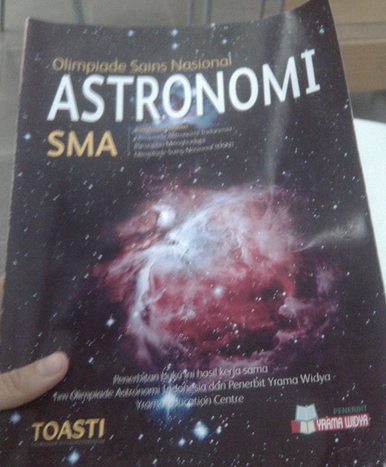
\includegraphics[width=0.5\textwidth]{gambar/buku_toasti.png}
\end{figure}
\begin{flushleft}
Sekitar sebulan lagi akan terbit ``Buku Sakti Olimpiade Astronomi'' persembahan TOASTI, jika kamu atau sekolah kamu tertarik bisa \textit{pre-order} lewat kontak di atas. 
\end{flushleft}

\end{document}
